\smallframetitle

\section{From 29/07/24 to 02/08/24}
\insertsectionframe

\subsection{Methodology for Identifying True Neighboring Base Stations Based on Antenna Azimuths}
\insertsubsectionframe


\begin{frame}
    \frametitle{Improved Methodology}
    The goal is to identify true neighboring base stations by analyzing antenna azimuths.
    \begin{block}{Azimuth approach}
        True neighbors are stations within each others line of sight and within the coverage range of their directed antennas.
    \end{block}
    \begin{block}{Defining Coverage Angles}
        \begin{itemize}
            \item \textbf{Antenna beamwidth}
            \begin{itemize}
                \item Each antenna has a specified azimuth and coverage angle (beamwidth).
                \item Coverage angles are calculated based on azimuth direction and beamwidth, giving start and end angles.
            \end{itemize}
            \item \textbf{Steps to Define Coverage Angles:}
            \begin{itemize}
                \item For an antenna with azimuth \( A \) and beamwidth \( B \):
                \begin{itemize}
                    \item Coverage Start Angle = \( A - \frac{B}{2} \)
                    \item Coverage End Angle = \( A + \frac{B}{2} \)
                \end{itemize}
            \end{itemize}
        \end{itemize}
    \end{block}
\end{frame}

\begin{frame}{Verification Process}
    \begin{block}{Step-by-Step Validation}
        \textbf{Step 1: Calculate the Direction of the Connecting Line:}
        \begin{itemize}
            \item Determine the azimuth angle of the line connecting the two base stations.
        \end{itemize}
        \textbf{Step 2: Validate Antenna Direction for Both Base Stations:}
        \begin{itemize}
            \item Check if the connecting line’s direction falls within the coverage angles of its antennas.
        \end{itemize}
        \textbf{Step 3: Determine the Shorter Angle:}
        \begin{itemize}
            \item Calculate the angle between the azimuth of the antenna and the direction of the connecting line.
            \item Measure the smaller angle between the azimuth and the connecting line direction.
        \end{itemize}
        \textbf{Step 4: Check Bi-Directional Coverage:}
        \begin{itemize}
            \item Perform validation from both base stations’ perspectives.
            \item If conditions are met for both, consider them true neighbors.
        \end{itemize}
        \textbf{Step 5: Applying the Distance Criterion:}
    \end{block}
\end{frame}

\begin{frame}{Analysis of Results}
    \begin{columns}
        \begin{column}{0.5\textwidth}
            \begin{figure}
                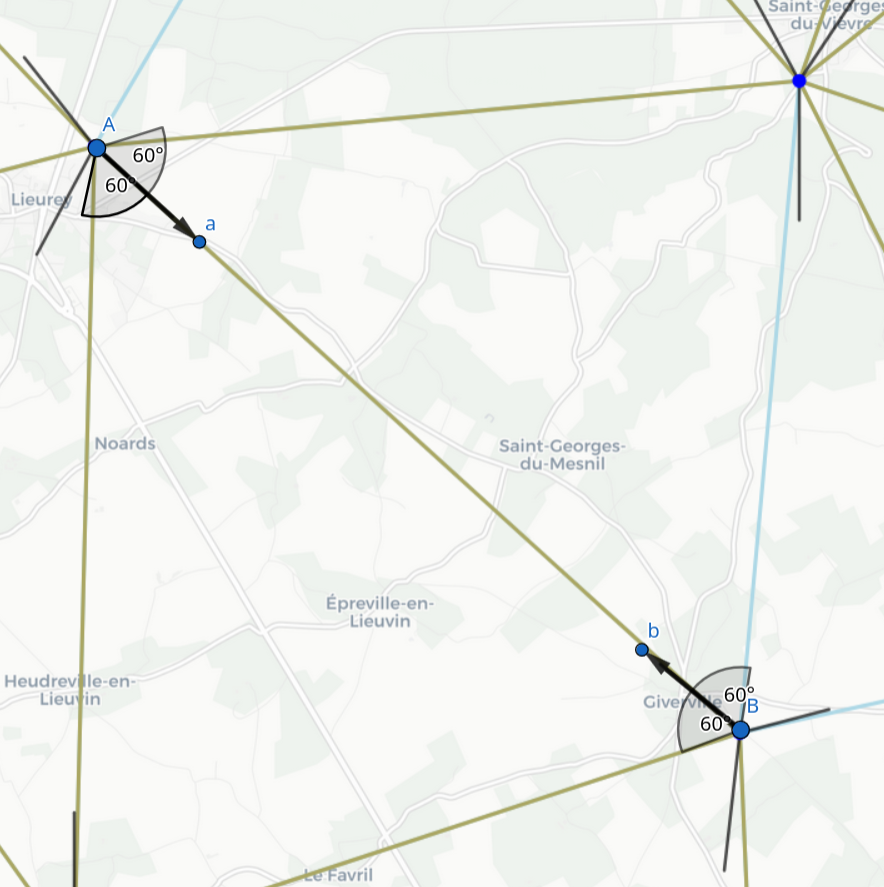
\includegraphics[height=0.3\paperwidth]{images/Altair/azimuth_expl.png}
                \caption{Visualization of the antenna coverage angle based methodology}
            \end{figure}
        \end{column}
        \begin{column}{0.5\textwidth}
            \begin{figure}
                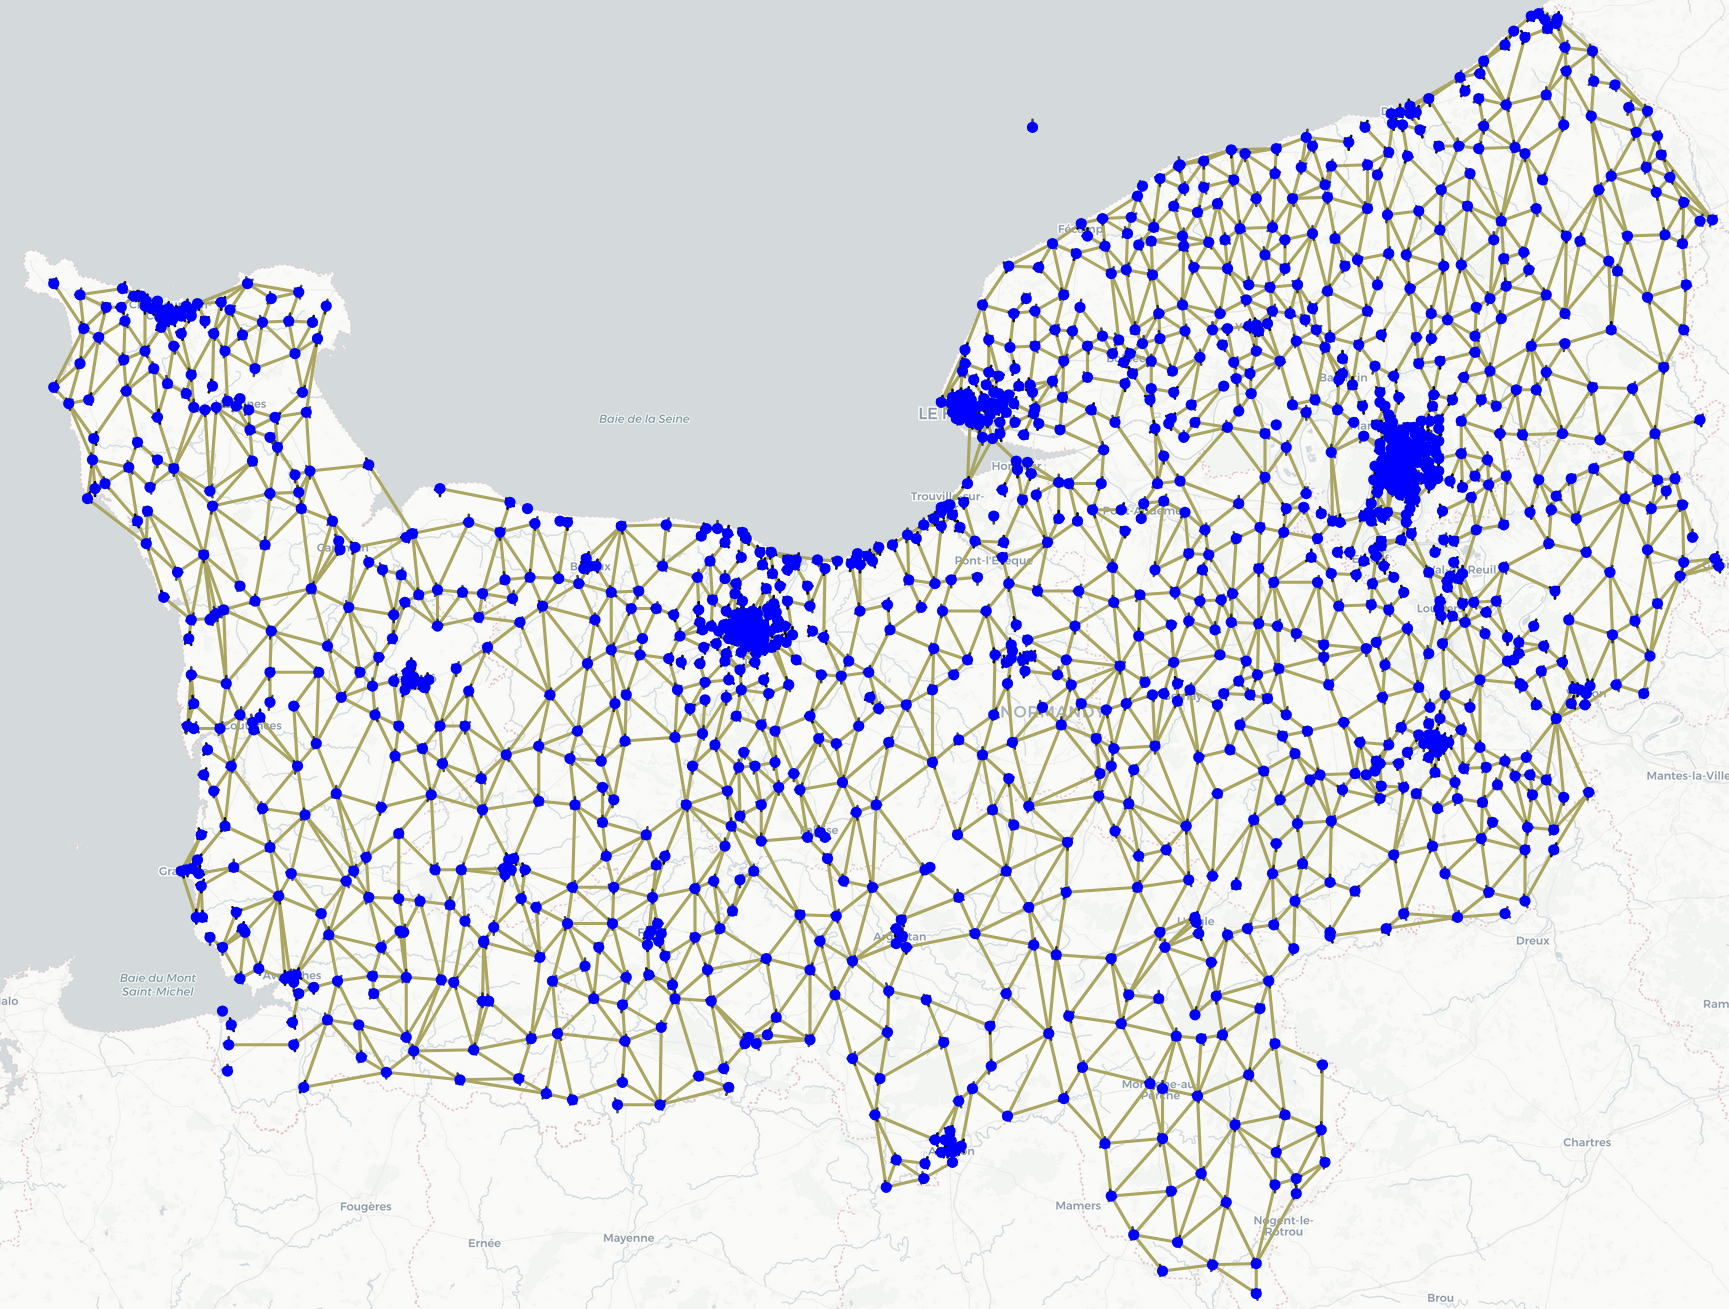
\includegraphics[height=0.6\paperheight]{images/Altair/azimuth_neigh_detect_normandy.png}
                \caption{Results on the map}
            \end{figure}
        \end{column}
    \end{columns}        
\end{frame}

\begin{frame}{Issue with Directional Antenna Coverage Methodology}
    \begin{columns}
        \begin{column}{0.5\textwidth}
            \begin{block}{Problem Explanation}
                \begin{itemize}
                    \item The current methodology focuses on identifying neighboring base stations based on the directional coverage of their antennas.
                    \item However, this approach can miss real neighboring stations that have overlapping coverage areas but whose antennas are not directly oriented towards each other.
                    \item As a result, some base stations that are effectively neighbors in terms of coverage might be excluded from the neighbor graph.
                    \item This limitation highlights the need for a more nuanced approach that considers not just the directional angles but also the actual coverage areas.
                \end{itemize}
            \end{block}
        \end{column}
        \begin{column}{0.5\textwidth}
            \begin{figure}
                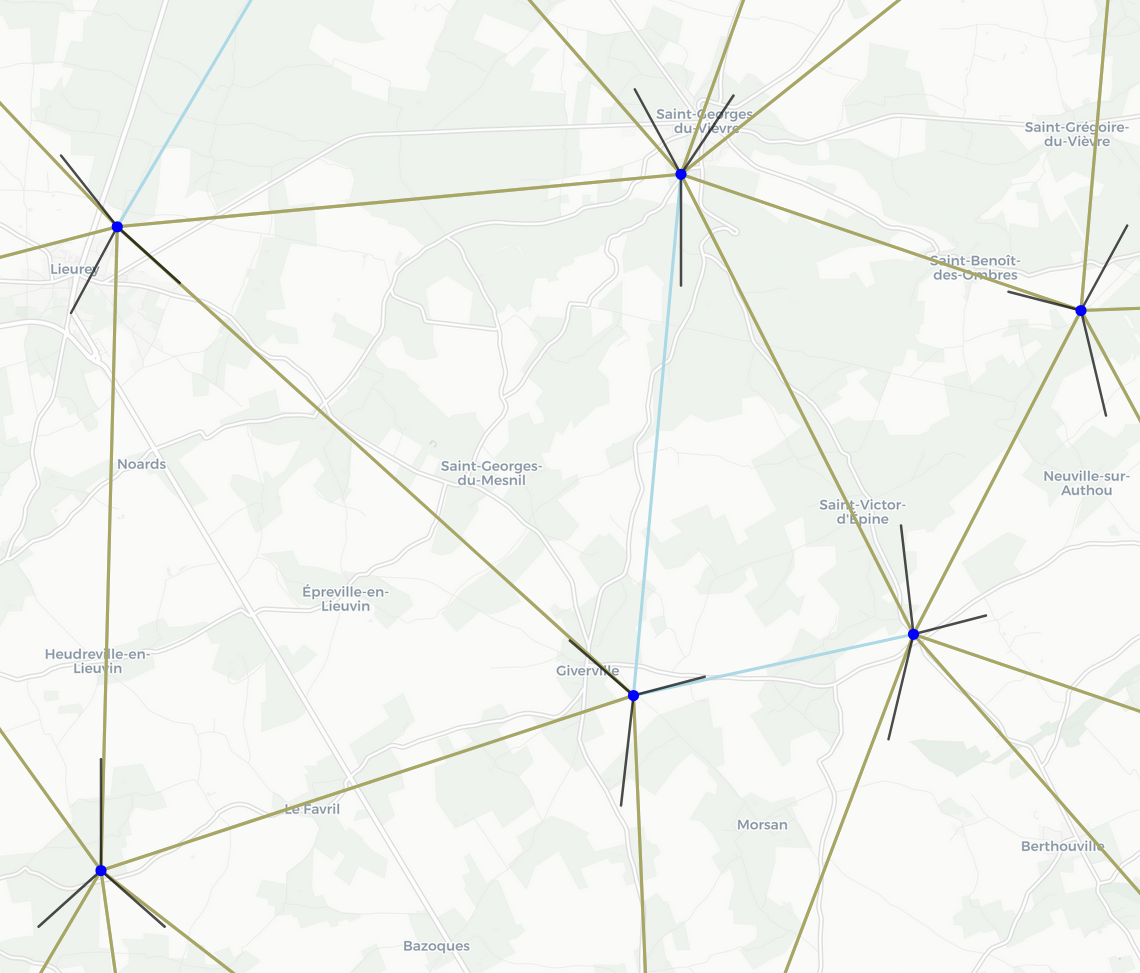
\includegraphics[width=0.7\textwidth]{images/Altair/problem_with_azimuth.png}  
                \caption{Coverage Overlap Issue}
            \end{figure}
        \end{column}
    \end{columns}
\end{frame}







